\documentclass{article}
\usepackage{amsfonts, amsmath, amssymb, amsthm, dsfont} % Math notations imported
\usepackage{enumitem}
\usepackage{graphicx}
\usepackage{setspace}
\usepackage{indentfirst}
\usepackage[margin=1in]{geometry}
\graphicspath{{./images/}} % Path to images

% \begin{figure}[htb!]
%      \centering
%      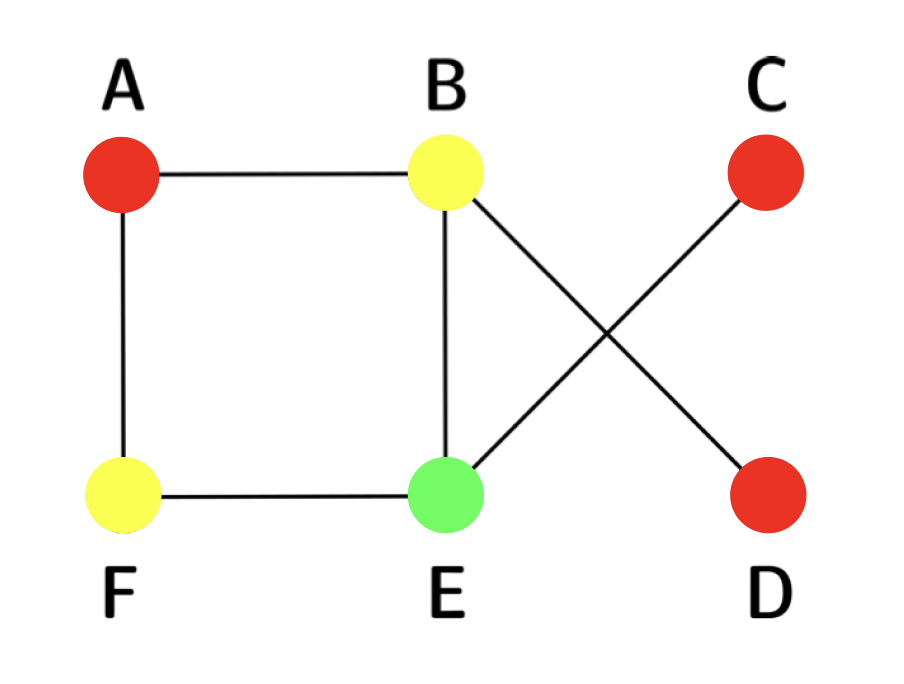
\includegraphics[scale=0.5]{coloring.png}
%      \caption{Coloring of the graph.}
% \end{figure}

% \begin{figure}[htb]
%     \qquad
%     \begin{minipage}{.4\textwidth}
%         \centering
%         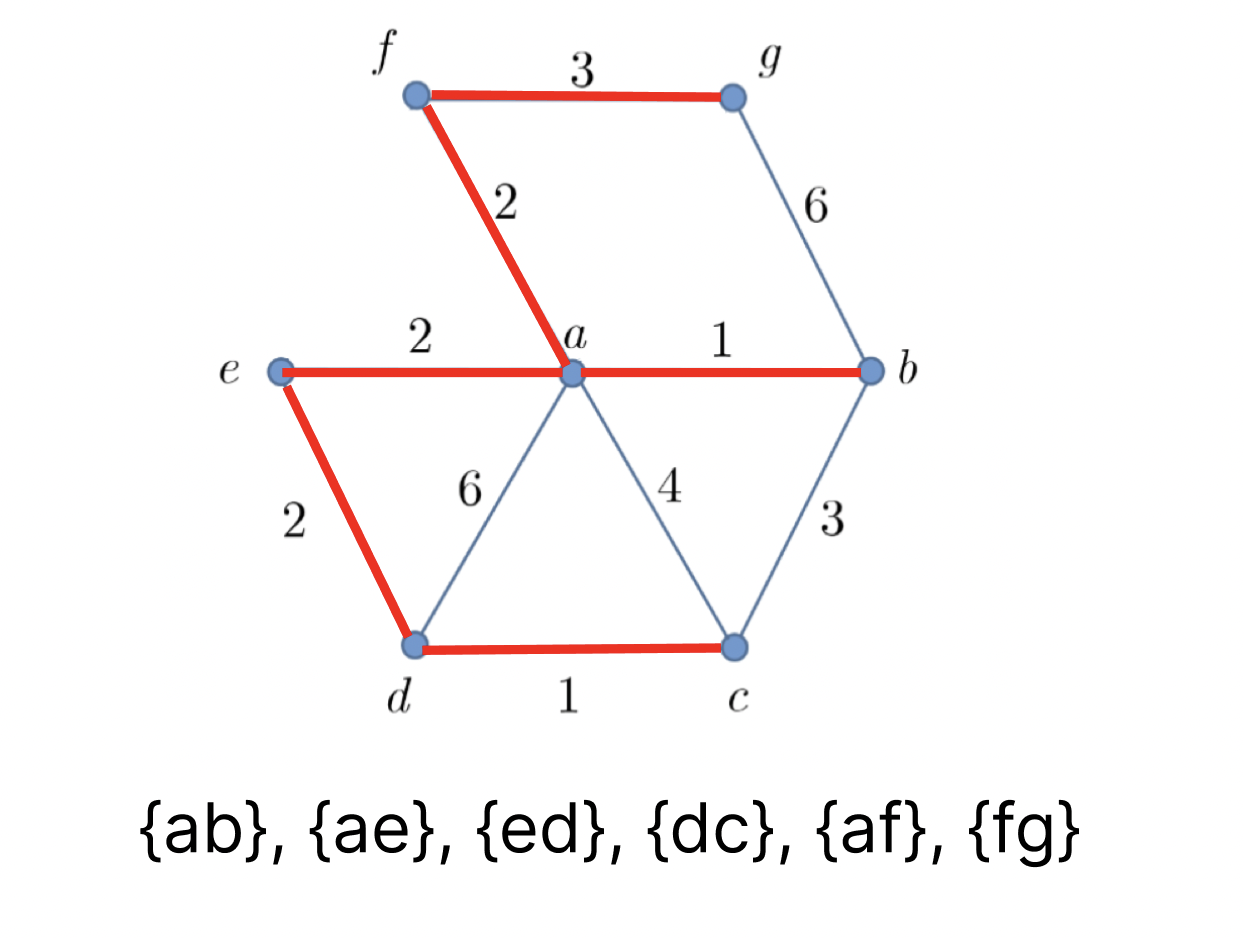
\includegraphics[scale=0.35]{prims.png}
%         \caption{}
%     \end{minipage}    
%     \qquad
%     \begin{minipage}{.4\textwidth}
%         \centering
%         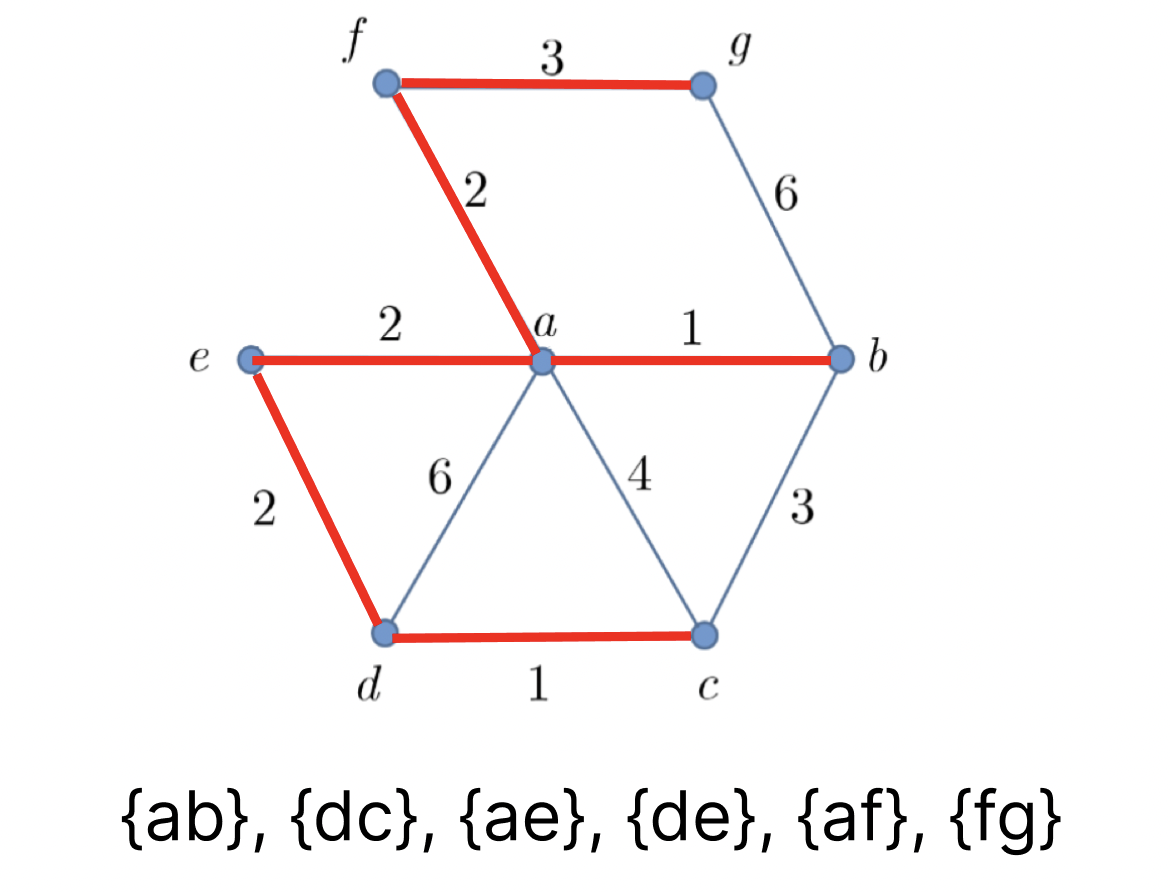
\includegraphics[scale=0.35]{kruskal.png}
%         \caption{}
%     \end{minipage}        
% \end{figure} 

\newtheorem{thm}{Theorem}
\newtheorem{proposition}[thm]{Proposition}
\newtheorem{corollary}[thm]{Corollary}
\newtheorem{lemma}[thm]{Lemma}

\newcommand*{\Var}{\ensuremath{\mathrm{Var}}}
\newcommand*{\Cov}{\ensuremath{\mathrm{Cov}}}
\newcommand*{\Corr}{\ensuremath{\mathrm{Corr}}}
\newcommand*{\Bias}{\ensuremath{\mathrm{Bias}}}
\newcommand*{\MSE}{\ensuremath{\mathrm{MSE}}}
\newcommand*{\range}{\ensuremath{\mathrm{range}}\,}
\newcommand*{\spann}{\ensuremath{\mathrm{span}}\,}
\newcommand*{\nul}{\ensuremath{\mathrm{null}}\,}
\newcommand*{\dom}{\ensuremath{\mathrm{dom}}\,}
\renewcommand*{\implies}{\ensuremath{\Longrightarrow}}
\renewcommand*{\impliedby}{\ensuremath{\Longleftarrow}}
\newcommand*{\Z}{\ensuremath{\mathbb{Z}}}
\newcommand*{\Q}{\ensuremath{\mathbb{Q}}}
\newcommand*{\R}{\ensuremath{\mathbb{R}}}
\newcommand*{\F}{\ensuremath{\mathbb{F}}}
\newcommand*{\C}{\ensuremath{\mathbb{C}}}
\newcommand*{\N}{\ensuremath{\mathbb{N}}}
\newcommand*{\E}{\ensuremath{\mathds{E}}}
\renewcommand*{\P}{\ensuremath{\mathds{P}}}
\newcommand*{\p}{\ensuremath{\mathcal{P}}}

% title information
\title{Math 110 HW11}
\author{Neo Lee}
\date{11/18/2023}

\setstretch{1.15}
% main content
\begin{document} 

% placing title information; comment out if using fancyhdr
\maketitle 

\subsection*{Problem 1.}
Find a polynomial $p\in {\cal P}_3(\R)$ such that
$$q'(1)=\int_0^1 p(t) q(t) dt \qquad {\rm for \; all} \;\; q\in {\cal P}_3(\R).$$
\begin{proof}[Solution]
    We only need to determine the action on the basis $q\in\{1, x, x^2, x^3\}$ because both 
    differentiation and integration are linear. For example, if $q = \alpha x^3 + \beta x^2 + 
    \gamma x + \delta$, then 
    \begin{align*}
        q'(1) & = \left(\alpha(x^3)' + \beta(x^2)' + \gamma(x)' + \delta(1)'\right)(1) \\
        & = \int_{0}^{1}\left(\alpha x^3\right)p(x)dx + \int_{0}^{1}\left(\beta x^2\right)p(x)dx + 
        \int_{0}^{1}\left(\gamma x\right)p(x)dx + \int_{0}^{1}\left(\delta\right)p(x)dx \\
        & = \int_{0}^{1}q(x)p(x)dx.
    \end{align*}

    Let $$p = ax^3 + bx^2 + cx + d,$$
    then we solve the system of linear equations
    \begin{align*}
        & \begin{cases}
            0 = \int_{0}^{1}\left(ax^3 + bx^2 + x + d\right)dx \\
            1 = \int_{0}^{1}\left(ax^4 + bx^3 + cx^2 + dx\right) dx \\
            2 = \int_{0}^{1}\left(ax^5 + bx^4 + cx^3 + dx^2\right) dx \\
            3 = \int_{0}^{1}\left(ax^6 + bx^5 + cx^4 + dx^3\right) dx
        \end{cases} \\
        \implies & \begin{cases}
            0 = \frac{1}{4}a + \frac{1}{3}b + \frac{1}{2}c + d \\
            1 = \frac{1}{5}a + \frac{1}{4}b + \frac{1}{3}c + \frac{1}{2}d \\
            2 = \frac{1}{6}a + \frac{1}{5}b + \frac{1}{4}c + \frac{1}{3}d \\
            3 = \frac{1}{7}a + \frac{1}{6}b + \frac{1}{5}c + \frac{1}{4}d
        \end{cases} \\
        \implies & \begin{cases}
            a = 1680 \\
            b = -2340 \\
            c = 840 \\
            d = -60
        \end{cases} \\
        \implies & p = 1680x^3 - 2340x^2 + 840x - 60.
    \end{align*}
\end{proof}

\newpage
\subsection*{Problem 2.}
Let $V=C[-\pi,\pi]$ with the inner product
$$\langle f, g \rangle := \int_{-\pi}^\pi f(t) \overline{g(t)} dt.$$
Determine the orthogonal projection of the function $h(x)=\exp(2ix)$ on the subspace
\begin{enumerate}[label=(\alph*)]
    \item $\spann (1, \cos x , \sin x)$; 
    \item $\spann (1,\cos x , \sin x, \cos 2x, \sin 2x)$; 
    \item $\spann (1,  \cos x , \sin x, \ldots, \cos nx, \sin nx)$ for $n>2$.
\end{enumerate}
\begin{proof}[Solution]\indent
    Notice $$h(x) = e^{2ix} = \cos(2x) + i\sin(2x),$$
    and all $$(1, \cos x, \sin x, \cos 2x, \sin 2x, \dots)$$ are orthogonal to each other (a property
    of Fourier Series).
    In fact, all the trig functions have length $\sqrt{\pi}$, so the orthonormal version would be 
    $$\left(\frac{1}{\sqrt{2\pi}}, \frac{\cos x}{\sqrt{\pi}}, \frac{\sin x}{\sqrt{\pi}},
    \frac{\cos 2x}{\sqrt{\pi}}, \frac{\sin 2x}{\sqrt{\pi}}, \dots\right),$$ but we don't need 
    to make use of the orthonormal version in this question.
    \begin{enumerate}[label=(\alph*)]
        \item $h(x)$ is orthogonal to all the basis because $\cos(2x), i(\sin 2x)$ are orthogonal 
        to the basis. So the projection is $0$.

        \item Notice $h(x)$ is in the span of the basis as noted in the very first line, so the
        projection is $h(x)$.

        \item Again, $h(x)$ is in the span of the basis, so the projection is $h(x)$.
    \end{enumerate}    
\end{proof}

\newpage
\subsection*{Problem 3.}
Find $p\in {\cal P}_3(\R)$  such that $p(-1)=0$, $p'(-1)=0$, and the following is minimized:
$$\int_0^1 (1-5x-p(x))^2 dx.$$
\begin{proof}
    Denote $$V = \{p\in\p_3(\R):p(-1)=0, p'(-1)=0\}.$$
    Let $p=ax^3+bx^2+cx+d$, then solving the equations 
    $$\begin{cases}
        0 = p(-1) \\
        0 = p'(-1)
    \end{cases}$$ yields
    $$\begin{cases}
        a = a \\
        b = b \\
        c = 2b-3a \\
        d = b-2a
    \end{cases},$$
    which implies $p = a(x^3-3x-2)+b(x^2+2x+1)\implies V = \spann\left\{(x+1)^3,(x+1)^2\right\}$.
    We want to find the orthogonal projection of $(1-5x)$ onto $V$, which would minimize the 
    integral.
    The orthonoaml basis are 
    \begin{align*}
        e_1 & = \frac{(x+1)^2}{\sqrt{\int_{0}^{1}(x+1)^4dx}} = \sqrt{\frac{5}{31}}(x+1)^2 \\
        e_2 & = \frac{(x+1)^3 - \frac{5}{31}(x+1)^2\int_{0}^{1}(x+1)^5dx}
        {\|(x+1)^3-\langle(x+1)^3, e_1\rangle e_1\|} \\
        & = \sqrt{\frac{868}{313}}\left((x+1)^3 - \frac{105}{62}(x+1)^2\right).
    \end{align*}
    Then the projection is 
    \begin{align*}
        P_u & = \langle (1-5x), e_1\rangle e_1 + \langle (1-5x), e_2\rangle e_2 \\
        & = \frac{-95}{124}(x+1)^2 - \frac{791}{626}\left((x+1)^3-\frac{105}{62}(x+1)^2\right) \\
        & = \frac{430}{313}(x+1)^2 - \frac{791}{626}(x+1)^3.
    \end{align*}
\end{proof}


\newpage
\subsection*{Problem 4.}
Find $p\in {\cal P}_3(\R)$  such that $p(-1)=0$, $p'(-1)=0$, and the following is minimized:
$$p(0)^2+\int_0^1 (1-5x-p'(x))^2 dx.$$
\begin{proof}[Solution]
    We can view this as minimizing the orthogonal residual of projecting $x-\frac{5}{2}x^2$ onto 
    $V$ where $$V = \spann\left\{(x+1)^2,(x+1)^2\right\},$$ 
    and the inner product is 
    $$\langle f,g\rangle=f(0)g(0)+\int_{0}^{1}f'(x)g'(x)dx.$$
    The orthonormal basis are
    \begin{align*}
        e_1 & = \frac{(x+1)^2}{\sqrt{1 + \int_{0}^{1}4(x+1)^2dx}} \\
        & = \sqrt{\frac{3}{31}}(x+1)^2 \\
        e_2 & = \frac{(x+1)^3 - \sqrt{\frac{3}{31}}(x+1)^2\left(\sqrt{\frac{3}{31}} + \sqrt{\frac{3}{31}}\int_{0}^{1}6(x+1)^3dx\right)}
        {\|(x+1)^3-\left\langle(x+1)^3, e_1\right\rangle e_1\|} \\
        & = \sqrt{\frac{620}{2081}}\left((x+1)^3 - \frac{141}{62}(x+1)^2\right).
    \end{align*}
    
    So the projection is 
    \begin{align*}
        P_u & = \left\langle \left(x-\frac{5}{2}x^2\right), e_1\right\rangle e_1 + 
        \left\langle \left(x-\frac{5}{2}x^2\right), e_2\right\rangle e_2 \\
        & = \frac{-16}{31}(x+1)^2 - \frac{1315}{2081}\left((x+1)^3 - \frac{141}{62}(x+1)^2\right) \\
        & = \frac{3833}{4162}(x+1)^2 - \frac{1315}{2081}(x+1)^3.
    \end{align*}
\end{proof}

\newpage
\subsection*{Problem 5.}
Let $V$ be the vector space $\R^3$ equipped with the standard inner product. 
Prove or disprove: any linear operator $P \in {\cal L}(V)$ such that $P^2=P$ is an orthogonal 
projector.
\begin{proof}[Solution]
    Define 
    $$T:(x,y,z)\mapsto(y,x,z).$$
    Consider $v=(1,2,3)$, then 
    $$\langle T(v), v - T(v)\rangle = \langle(2,1,3), (-1,1,0)\rangle = -1\neq 0,$$
    which means the residual is not orthogonal to the image of $T$, so $T$ is not an orthogonal 
    projector.
\end{proof}

\end{document}
